% Created 2015-10-05 Mon 13:46
\documentclass[11pt]{article}
\usepackage[utf8]{inputenc}
\usepackage[T1]{fontenc}
\usepackage{fixltx2e}
\usepackage{graphicx}
\usepackage{grffile}
\usepackage{longtable}
\usepackage{wrapfig}
\usepackage{rotating}
\usepackage[normalem]{ulem}
\usepackage{amsmath}
\usepackage{textcomp}
\usepackage{amssymb}
\usepackage{capt-of}
\usepackage{hyperref}
\date{\today}
\title{Analyse III}
\hypersetup{
 pdfauthor={},
 pdftitle={Analyse III},
 pdfkeywords={},
 pdfsubject={},
 pdfcreator={Emacs 24.5.1 (Org mode 8.3.2)}, 
 pdflang={English}}
\begin{document}

\maketitle
\tableofcontents


\section{Chapitre 1}
\label{sec:orgheadline9}
\uline{\textbf{Opérateurs différentiels de la physique}}
\subsection{Def: Gradient (\(\nabla\))}
\label{sec:orgheadline1}
Gradient : \(\mathbb{R}^n \rightarrow \mathbb{R}^n\)

\(\text{grad} f(x) = \nabla f(x) = \left(\frac{\delta f}{\delta x_1}
(x),...,\frac{\delta f}{\delta x_n} (x)\right) \in \mathbb{R^n}\)
\subsection{Def: Laplacien (\(\Delta\))}
\label{sec:orgheadline2}
Laplacien : \(\mathbb{R}^n \rightarrow \mathbb{R}\)

\(\Delta f(x) = \sum\limits_{i=1}^n \frac{\delta^2 f}{\delta x_i^2} (x) \in \mathbb{R}^2\)
\subsection{Def: Champ vectoriel (\(F\))}
\label{sec:orgheadline3}
Champ vectoriel : \(\mathbb{R}^n \rightarrow \mathbb{R}^n\)

\(F(x) = \left(F_1(x),...,F_n(x)\right)\)

\(F_i: \mathbb{R}^n \rightarrow \mathbb{R}\)
\subsection{Def: Divergence (\(div\) ou \(\nabla\).)}
\label{sec:orgheadline4}
Divergence : \(\mathbb{R}^n \rightarrow \mathbb{R}\)


\(\text{div} F = \nabla . F = \sum\limits_{i=1}^n \frac{\delta F_i}{\delta x_i}\)
\subsection{Def: Rotationnel (\(rot\) ou  \(\Delta \times\))}
\label{sec:orgheadline7}
Rotationnel : \(\mathbb{R}^n \rightarrow \mathbb{R}^{\frac{n(n-1)}{2}}\)
\subsubsection{Pour n=2}
\label{sec:orgheadline5}
\(F: \mathbb{R}^2 \rightarrow \mathbb{R}^2\), \(F=(F_1,F_2)\)

\(\text{rot} F = \Delta \times F = \frac{\delta F_2}{\delta x_1} - \frac{\delta
F_1}{\delta x_2} \in \mathbb{R}\)

\(\left(= \begin{vmatrix}
\frac{\delta}{\delta x_1} & \frac{\delta}{\delta x_2}\\
F_1 & F_2
\end{vmatrix}\right)\)
\subsubsection{Pour n=3}
\label{sec:orgheadline6}
\(F: \mathbb{R}^3 \rightarrow \mathbb{R}^3\), \(F=(F_1,F_2,F_3)\)

\(\text{rot} F = \Delta \times F = \left( \frac{\delta F_3}{\delta x_2} -
\frac{\delta F_2}{\delta x_3},\frac{\delta F_1}{\delta x_3} - \frac{\delta
F_3}{\delta x_1}, \frac{\delta F_2}{\delta x_1} - \frac{\delta F_1}{\delta x_2}
\right) \in \mathbb{R}^3\)

\(\left(= \begin{vmatrix}
\frac{\delta}{\delta x_1} & \frac{\delta}{\delta x_2}& \frac{\delta}{\delta x_3}\\
F_1 & F_2 & F_3
\end{vmatrix}\right)\)
\subsection{Propriétés}
\label{sec:orgheadline8}
\begin{enumerate}
\item \(\Delta f = \text{div}(\text{grad} f) = \nabla . (\nabla f)\)
\item \(f : \mathbb{R}^n \rightarrow \mathbb{R}\) et \(F: \mathbb{R}^3 \rightarrow
   \mathbb{R}^3\) \textbf{\(n=3\)} \(\text{rot}(\nabla f) =0 \in \mathbb{R}^3\), \(\text{div(rot} F) =
   0\) pour \textbf{\(n=2\)} \(\text{rot}(\nabla) = 0 \in \mathbb{R}\)
\item \(\text{div}(f\nabla g) = f \Delta g + \nabla f \nabla g\)
\item \(\nabla(fg) = g \nabla f + f \nabla g\)
\item \(\text{div}(fF) = f \text{div} F + \nabla f F\)
\item \(\text{rot rot} F = - \Delta F + \nabla \text{div} F\)
\end{enumerate}
\section{Chapitre 2}
\label{sec:orgheadline27}
\uline{\textbf{Intégrales curvilignes}}
\subsection{Def: Courbe simple}
\label{sec:orgheadline15}
\(\Gamma \subset \mathbb{R}^d\) est une courbe simple si \(\exists I \subset
\mathbb{R}\)  (intervalle) et \(\gamma: I \rightarrow \mathbb{R}^d\) : continue. tel que
\begin{enumerate}
\item \(\gamma (I) = \tau\) (courbe)
\item \(\gamma (t_1) \neq \gamma(t_2)\) \(\forall t_1,t_2 \in I\) (simple)
\end{enumerate}
\(\gamma\) : une paramétrisation.

\subsubsection{Ex. 1 : Cercle}
\label{sec:orgheadline10}
\(\Gamma = \{ x \in \mathbb{R}^2 : |x|=1\}\) dessin cercle \(\gamma:
    \left[0,2\pi\right] \rightarrow \mathbb{R}^2\) \(\gamma(\theta) = (\cos
    \theta, \sin \theta)\)
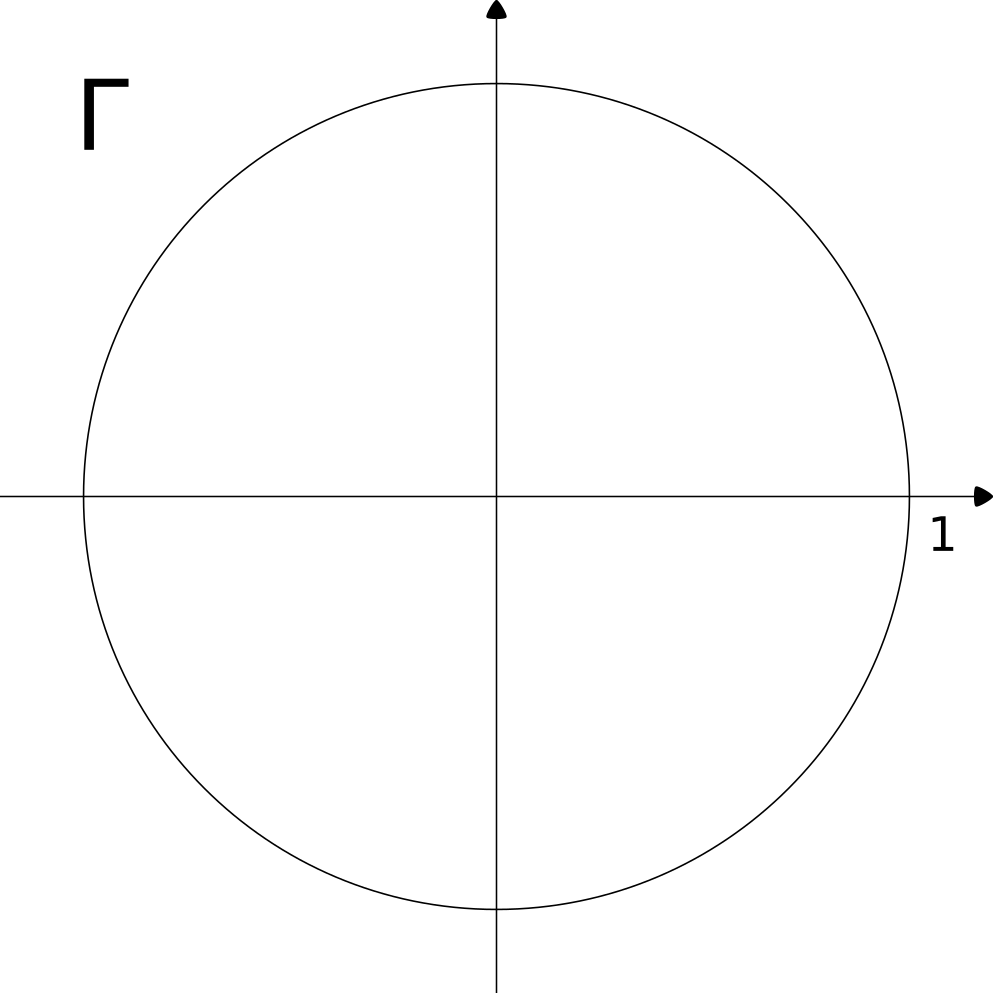
\includegraphics[width=.9\linewidth]{images/an_ch2_ex_1.png}
\subsubsection{Ex. 2 : Helix}
\label{sec:orgheadline11}
\(\gamma \mathbb{R} \rightarrow \mathbb{R}^3\) \(\gamma(t) = (\cos t, \sin t,t)\)
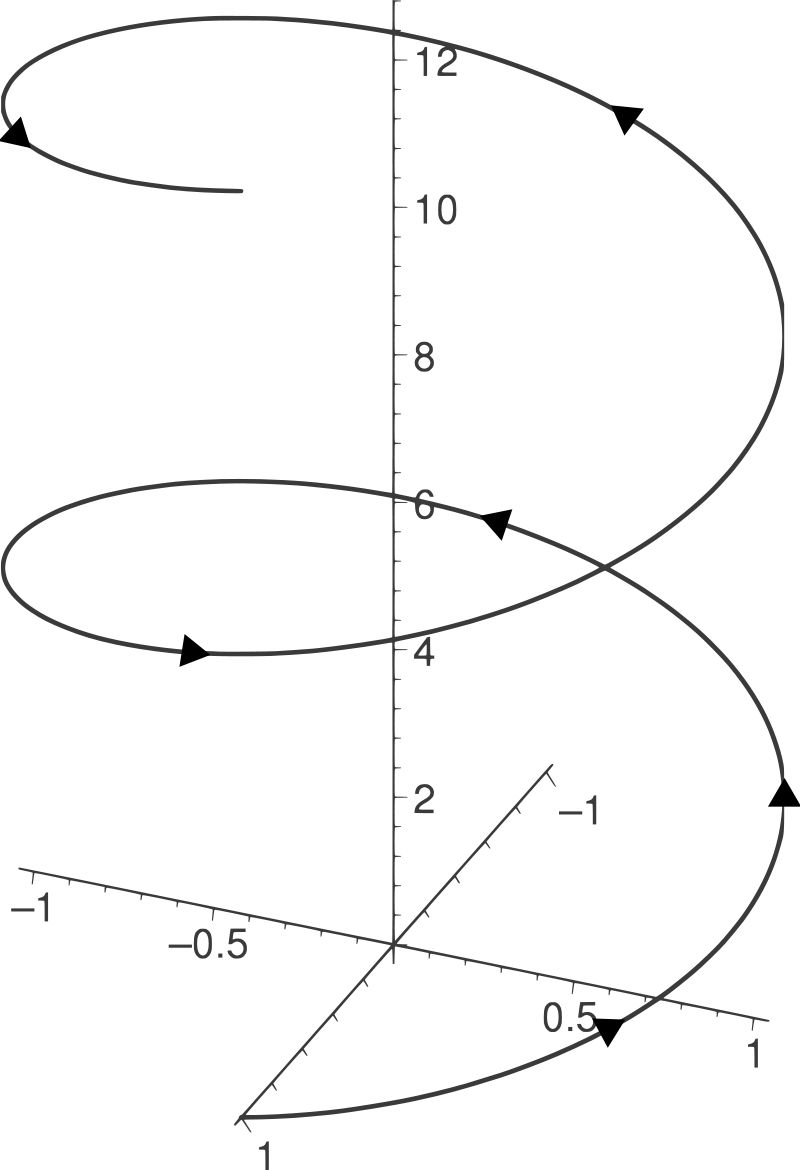
\includegraphics[width=.9\linewidth]{images/an_ch2_ex_2.png}
\subsubsection{Ex. 3 : Puissances}
\label{sec:orgheadline12}
\(\mathbb{R} \rightarrow \mathbb{R}^2\) \(\gamma(t) = (t^3,t^2)\)
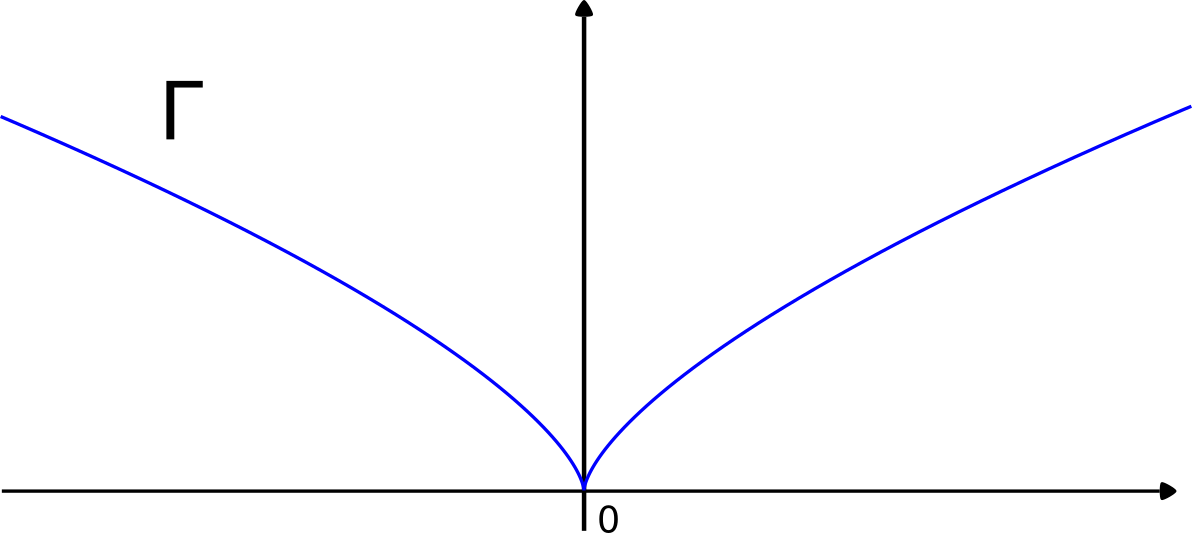
\includegraphics[width=.9\linewidth]{images/an_ch2_ex_3.png} 
\subsubsection{Ex. 4: Valeur absolue}
\label{sec:orgheadline13}
\(\gamma : \mathbb{R} \rightarrow \mathbb{R}^2\) \(\gamma(t) = (t,|t|)\) dessin
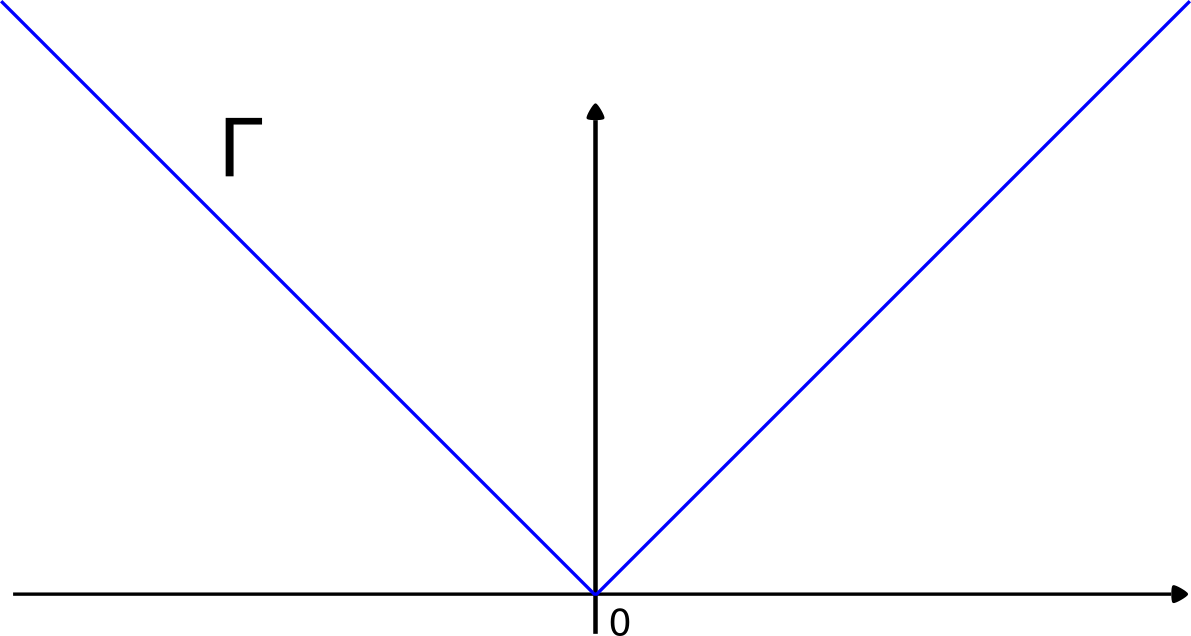
\includegraphics[width=.9\linewidth]{images/an_ch2_ex_4.png}
\subsubsection{Ex. 5 : Courbe "complexe"}
\label{sec:orgheadline14}
\(\mathbb{R}^2\) courbe pas simple
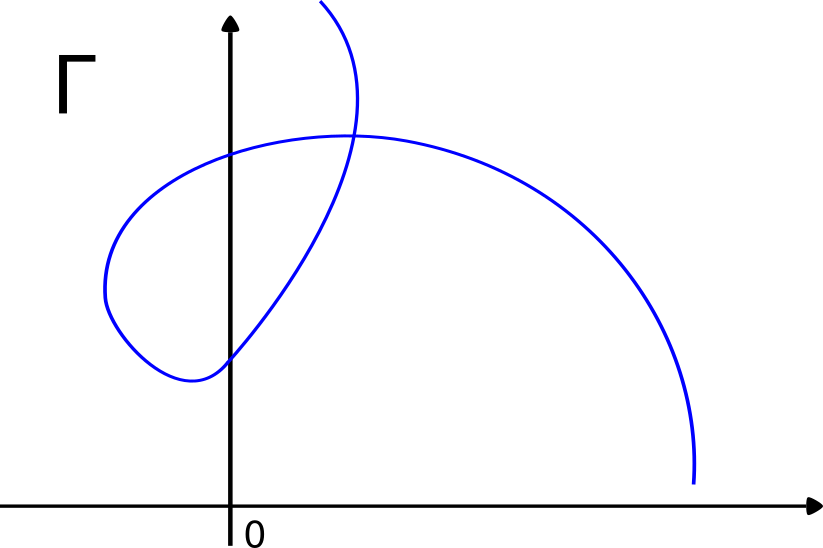
\includegraphics[width=.9\linewidth]{images/an_ch2_ex_5.png}

\subsection{Def 2 :  Courbe simple fermée}
\label{sec:orgheadline16}
\(\tau\) : courbe simple est dite fermée si \(\gamma(a) = \gamma(b)\) \(\left(I = \left[a,b\right]\right)\)
\begin{itemize}
\item Ex. \hyperref[sec:orgheadline10]{1} : fermé \(\gamma(0)=\gamma(2\pi) = (1,0)\) image patate.
\item Ex. \hyperref[sec:orgheadline11]{2},\hyperref[sec:orgheadline12]{3},4 : non fermé.
\end{itemize}

\subsection{Def 3: Courbe régulière}
\label{sec:orgheadline18}
\(\Gamma\) : courbe est régulière si \(\exists \left[a,b\right], \gamma: \gamma \cdot \left[a,b\right] \rightarrow \mathbb{R}^d\) tel que
\begin{itemize}
\item \(\gamma \in C^1 \left(\left[a,b\right]: \mathbb{R}^2\right)\)
\item \(\gamma ' (t) \neq 0 \in \mathbb{R}^d\) \(\left( \left(\gamma_1'(t),...,\gamma_d'(t) \right) \neq (0,...,0) \right)\)
\end{itemize}
\begin{itemize}
\item \hyperref[sec:orgheadline10]{Ex.1} : régulière \(\gamma'(t) = (-\sin t, cos t) \neq (0,0)\)
\item \hyperref[sec:orgheadline11]{Ex.2} : régulière \(\gamma'(y) = (-\sin t, cos t, 1) \neq (0,0,0)\)
\item \hyperref[sec:orgheadline12]{Ex.3} : \(\gamma' (t) = (3t^2,2t)\) et \(\gamma'(0) = (0,0)\) : \(\Gamma\) : n'est pas régulière.
\item Ex.4 : \(\gamma\) n'est pas diff. en \(t=0\). Donc \(\Gamma\) n'est pas régulière.
\end{itemize}

\subsubsection{Remarque :}
\label{sec:orgheadline17}
\begin{itemize}
\item \(\Gamma\) : régulière. La ligne tangente en \(\gamma(t_0)\):
\end{itemize}
(L) : \(\gamma(t_0) + \gamma'(t_0)(t-t_0)\)

\begin{itemize}
\item \(\Gamma\) : courbe \(\subset \mathbb{R}^d\)
\end{itemize}

\(f: \Gamma \rightarrow \mathbb{R}\): continue.

\subsection{Def : \(\int\limits_{\Gamma} f\)}
\label{sec:orgheadline22}
\(\int\limits_{\Gamma} f := \int\limits_{a}^{b} f(\gamma(t)) ||\gamma'(t)|| dt\)

\(\gamma : \left[a,b\right] \rightarrow \mathbb{R}^d\): une paramétrisation de \(\Gamma\).

La longueur de \(\Gamma\) : \(\int\limits_{\Gamma} 1 = \int\limits_{a}^{b}||\gamma'(t)|| dt\)

\subsubsection{Retour à \hyperref[sec:orgheadline10]{ex. 1}. :}
\label{sec:orgheadline19}
\(\int\limits_{\Gamma}f\) avec \(f=1\)

\(= \int\limits_{0}^{2\pi} ||\gamma'(t)|| dt = \int\limits_{0}^{2\pi} 1 dt = 2\pi\)

\subsubsection{Ex. :}
\label{sec:orgheadline20}
\begin{align*}
\int\limits_{\Gamma} : f(x,y) = \sqrt{x^2+4y^2}
\end{align*}
\begin{align*}
\Gamma = \left\lbrace (x,y) \in \mathbb{R}^2; 2y = x^2; x \in \left[0,1\right]\right\rbrace
\end{align*}
\begin{align*}
\gamma : \left[0,1\right] \rightarrow \mathbb{R}^2\\
t \rightarrow (t,\frac{t^2}{2})
\end{align*}
\begin{align*}
\int\limits_{\Gamma} f &= \int\limits_{0}^{1} f(\gamma(t)) || \gamma'(t)|| dt\\
&= \int\limits_{0}^{1} \sqrt{t^2 + 4 \frac{t^4}{4}} \sqrt{1 + t^2} dt\\
&= \int\limits_{0}^{1} \sqrt{t^2 + t^4} \sqrt{1 + t^2} dt\\
&= \int\limits_{0}^{1} t (1+t^2) dt = \frac{t^2}{2} + \frac{t^4}{4} \big|_0^1= \frac{3}{4} 
\end{align*}

\subsubsection{Somme intégrale}
\label{sec:orgheadline21}

\begin{align*}
\int\limits_{\Gamma}f \simeq \sum\limits_i |\Gamma_i| f(\gamma(t_i))\\
\gamma(t_i) \in \Gamma_i \\
\simeq \sum\limits_i |\Gamma_i| f(\gamma(t_i))\\
\end{align*}
\(\Gamma_i = \gamma \left( \left[ t_i, t_{i+1} \right] \right)\): \(\gamma\) une paramétrisation \(\left[a,b\right] \rightarrow \mathbb{R}^d\)

Donc \(\int\limits_{\Gamma}f \simeq \sum\limits ||\gamma(t_i)'|| (t_{i+1} - t_i) f(\gamma(t_i)) \simeq \int\limits_{a}^{b} ||\gamma'(t)|| f(\gamma(t)) dt\)

\((t_1) \neq \gamma(t_2)\) \(\forall t_1,t_2 \in I\) (simple)
\(\gamma\) : une paramétrisation.

\subsection{Def : L'intégrale curviligne pour un champ vectoriel.}
\label{sec:orgheadline23}

\(F : \Gamma \rightarrow \mathbb{R}^d\)
\(\Gamma\) : courbe \(\gamma\) : paramétrisation sur \(\left[a,b\right]\)
\(\int\limits_{\Gamma} F \vec{dl} := \int\limits_{a}^{b} F(\gamma(t))\cdot\gamma'(t) dt\) (\(\cdot\) =produit scalaire\ldots{})

\begin{itemize}
\item Ex : \(\int\limits_{\Gamma} F \vec{dl}\)
\end{itemize}
\(\Gamma = \left\lbrace (x,y) \in \mathbb{R}^2: y = \cosh x, x \in \left[0,1\right] \right\rbrace\)

\(F(x,y) = (x^2,0)\ \ \gamma: \left[0,1\right] \rightarrow \mathbb{R}^2\)

\(\gamma(t) = (t,\cosh t)\)
\(\int\limits_{\Gamma} F \vec{dl}\)
\begin{align*}
\Gamma &=  \int\limits_{0}^{1} F(\gamma(t)) \cdot \gamma'(t) dt = \int\limits_{0}^{1} (t^2,0)\cdot(1,\sinh t) dt\\
&= \int\limits_{0}^{1} t^2 dt = \frac{1}{3}
\end{align*} 

\subsection{Def : courbe régulière \underline{par morceau}.}
\label{sec:orgheadline24}
\(\exists \gamma \left[a,b\right] \rightarrow \mathbb{R}^d\)
\(t_0=a,...,t_k=b\)
tel que : \(\gamma \in C^1 \left(\left[t_i,t_{i+1}\right]\right)\)
\(\gamma'(t) \neq 0\ \forall t \neq t_i\)

\subsection{Def : \(\Gamma\) régulière \underline{par morceau}:}
\label{sec:orgheadline26}
\(f : \Gamma \rightarrow \mathbb{R}\): continue.
\begin{align*}
\int\limits_{\Gamma} f := \sum\limits_{i=0}^{k-1} f(\gamma(t)) || \gamma'(t)|| dt
\end{align*}
\(F: \Gamma \rightarrow \mathbb{R}^d\) : champ vectoriel:
\begin{align*}
\int\limits_{\Gamma}F \vec{dl} := \sum\limits_{i=0}^{k-1} \int\limits_{t_i}^{t_{i+1}} F(\gamma(t)) || \gamma'(t)|| dt
\end{align*}

\subsubsection{Ex. : Périmètre d'un carré}
\label{sec:orgheadline25}
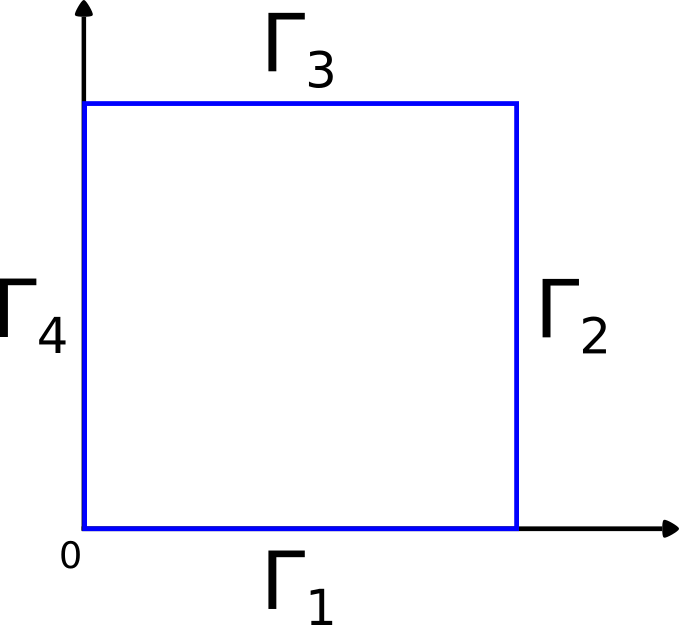
\includegraphics[width=.9\linewidth]{images/an_ch2_ex_6.png}
\(\Gamma = \Gamma_1 \cup \Gamma_2 \cup \Gamma_3 \cup \Gamma_4\)
\begin{align*}
\Gamma_1 &= \left\lbrace (t,0): t\in \left[0,1\right] \right\rbrace\\
\Gamma_2 &= \left\lbrace (1,t-1): t\in \left[1,2\right] \right\rbrace\\
\Gamma_3 &= \left\lbrace (3-t,1): t\in \left[2,3\right] \right\rbrace\\
\Gamma_4 &= \left\lbrace (0,4-t): t\in \left[3,4\right] \right\rbrace\\
\end{align*}
\(\gamma: \left[0,4\right] \rightarrow \mathbb{R}^2\)
\begin{align*}
\gamma(t) = &\gamma_1(t) &\left[0,1\right]\\
 & \gamma_2(t) &\left[1,2\right]\\
 & \gamma_3(t) &\left[2,3\right]\\
 & \gamma_4(t) &\left[3,4\right]
\end{align*}


\(f=1\)
\begin{align*}
|\Gamma| = \int\limits_{\Gamma} f &= \int\limits_{0}^{1} || \gamma'(t)|| dt + \int\limits_{1}^{2} || \gamma'(t)|| dt\\
&+ \int\limits_{2}^{3} || \gamma'(t)|| dt  + \int\limits_{3}^{4} || \gamma'(t)|| dt\\
\end{align*}
\begin{align*}
(||\gamma'(t)||=1) = \int\limits_{0}^{1} 1 + \int\limits_{1}^{2} 1 + \int\limits_{2}^{3} 1 + \int\limits_{3}^{4} = 4
\end{align*}
\begin{align*}
\int\limits_{\Gamma}f= \sum\limits_{i=1}^4 \int\limits_{\Gamma_i}\\
\Gamma_2 : \left\lbrace (1,t) t \in \left[0,1\right] \right\rbrace
\end{align*}

\section{Chapitre 3}
\label{sec:orgheadline41}
\uline{\textbf{Champs qui dérivent d'un potentiel}}
\subsection{Def:}
\label{sec:orgheadline29}
\(\Omega\) ouvert \(\mathbb{R}^n\)

\(F: \Omega \rightarrow \mathbb{R}^n\)

\(F(x) = (F_1(x),...,F_n(x))\)

On dit que \(F\) dérive d'un potentiel sur \(\Omega\). Si \(\exists f: \Omega \rightarrow \mathbb{R}\)

\(f\in C^1(\Omega): \nabla f = F ds \Omega\)
\subsubsection{Exemple}
\label{sec:orgheadline28}
\(F(x) = x\)

\(f(x) = \frac{1}{2} ||x||^2 = \frac{1}{2} \sum\limits_{i=1}^n x_i^2\)

\(\nabla f = F\)

\(F\): dérive d'un potentiel.
\subsection{Théorème}
\label{sec:orgheadline31}
\(F\) dérive d'un potentiel,

\(F \in C^1(\Omega)\) Alors

\(\frac{\delta F_i}{\delta x_j}(x) = \frac{\delta F_j}{\delta x_i}(x) \forall i,j \in \lbrace 1,...,n\rbrace,\ \forall x \in \Omega\)
\subsubsection{Preuve}
\label{sec:orgheadline30}
\(F\) dérive d'un potentiel de \(f\)

\(f\) \(\in\) C\(^{\text{1}}\)(\(\Omega\))\$

\(\nabla f(x)= F(x) \forall x \in \Omega\)

Car \(F\in C^1(\Omega)\) on a

\(f \in C^2(\Omega)\)

Donc \(\frac{\delta^2 f}{\delta x_i \delta x_j}(x) = \frac{\delta^2 f}{\delta x_j \delta x_i}(x)\) \(\forall i,j \in \lbrace 1,...,n\rbrace,\ \forall x \in \Omega\) (1)

On a

\(F_i(x) = \frac{\delta f}{\delta x_i}(x)\) \(\forall x \in \Omega,\ \forall i\)

\(\frac{\delta^2 f}{\delta x_j}(x) = \frac{\delta^2 f}{\delta x_j \delta x_i}(x)\)  \(\forall x \in \Omega,\ \forall i,j\) (2)

\(\frac{\delta^2 f}{\delta x_i}(x) = \frac{\delta^2 f}{\delta x_i \delta x_j}(x)\)  \(\forall x \in \Omega,\ \forall i,j\) (3)

(1) (2) (3) \(\Rightarrow \frac{\delta F_i}{\delta x_j}(x) = \frac{\delta F_j}{\delta x_i}(x)\) 
\subsection{Question:}
\label{sec:orgheadline33}
F: régulier, suppossons \(\frac{\delta F_i}{\delta x_j}=\frac{\delta F_j}{\delta x_i}\) \(\forall x \in \Omega,\ \forall i,j\)

Est-ce que \(F\) dérive d'un potentiel ?
\subsubsection{Réponse}
\label{sec:orgheadline32}
Vrai si \(\Omega\) convexe ou simplement connexe.

"pas vrai": si \(\Omega\) n'est pas simplement connexe.
\subsection{Théorème}
\label{sec:orgheadline35}
\(\Omega\): ouver connexe

\(F: \Omega \rightarrow \mathbb{R}^n: F\in C(\Omega,\mathbb{R}^n)\)

Les affirmations suivantes sont équivalentes :
\begin{enumerate}
\item \(F\) dérive d'un potentiel
\item \(\int\limits_\Gamma F dl = 0\) \(\forall F\): fermée, régulière, par morceaux, dans \(\Omega\)
\end{enumerate}

\subsubsection{Preuve}
\label{sec:orgheadline34}
(1) \(\Rightarrow\) (2)

\(F\): dérive d'un potentiel

\(\exists f \in C^1(\Omega)\): \(\nabla f(x) = F(x)\) \(\forall x \in \Omega\)

\(\Gamma\): courbe fermée régulière.

\(\gamma: [a,b]:\) \(\Gamma = \gamma([a,b])\) et \(\gamma(a)=\gamma(b)\)

On calcule 

\begin{align*}
 \int\limits_{\Gamma} F \vec{dl} &= \int\limits_a^b F(\gamma (t)) \gamma'(t) dt\\
  &= \int\limits_a^b \nabla f(\gamma(t)) \gamma'(t) dt \\
&= \int\limits_a^b \frac{d}{dt} \left[ f(\gamma(t)) \right] dt\\
&= f(\gamma(b)) - f(\gamma(a)) = 0
\end{align*}


(2) \(\Rightarrow\) (1)

On sait :

\(\int\limits_{\Gamma} F \vec{dl} = 0\) \(\forall \Gamma\) fermée régulière.

\(\Omega\) \href{https://fr.wikipedia.org/wiki/Ensemble_convexe}{convexe}.

On montre \(\bar{f}\) dérive d'un potentiel

On va essayer de trouver \(f\) tel que

\(\nabla f = F\)

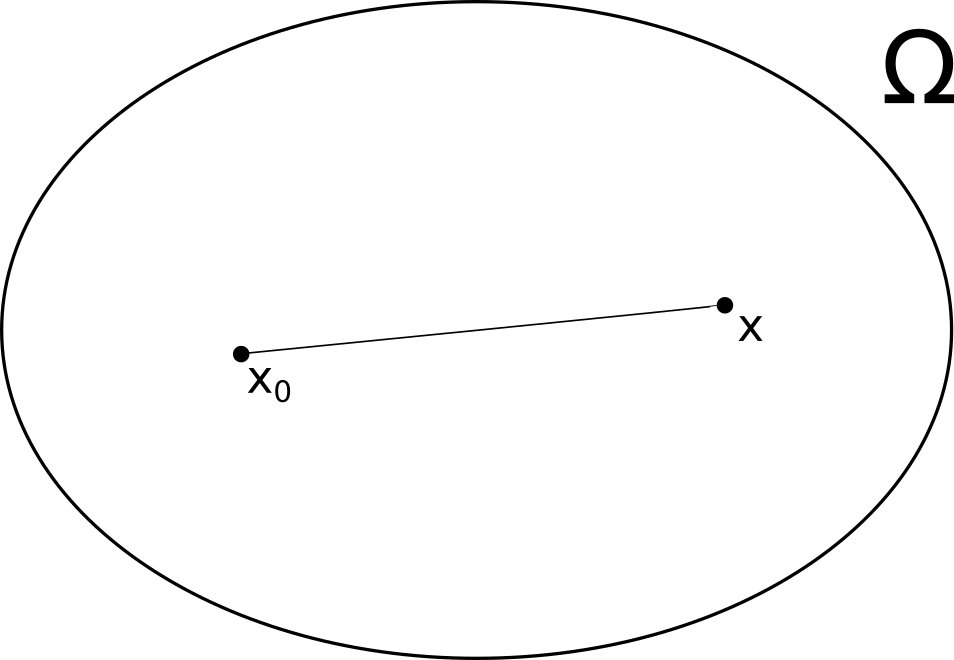
\includegraphics[width=.9\linewidth]{images/an_ch3_01.png}

On fixe : \(x_0 \in \Omega\).

Pour \(x \in \Omega\), \([x_0,x] = x_0 + t(x-x_0\) \(t \in [0,1]\) 

Définition : \(f(x) = \int\limits_{[x_0,x]} F \vec{dl}\)

\(\Omega\) convexe \(\Rightarrow [x_0,x] \subset \Omega\) \(\forall x \in \Omega\)

On montre:

\(\nabla f(x) = F(x)\) \(\forall x \in \Omega\)

\uline{Rappel}

\(f(y) - f(x) = \nabla f(x)(y-x)+o(||y-z||)\)

\(f(y) - f(x) = \int\limits_{[x_0,y]} F dl - \int\limits_{[x_0,x]} F dl\)

On a

\(\int\limits_{[x_0,x]} F dl + \int\limits_{[x,y]} F dl + \int\limits_{[y,x_0]} F
dl = 0\)

Donc :

\begin{align*}
f(y) -f(x) &= \int\limits_{[x_0,y]} + \int\limits_{[x,y]} + \int\limits_{[y,x_0]}\\
&= \int\limits_{[x,y]} F \vec{dl}
\end{align*}

\([x,y] = \lbrace x+ t(y-x): t\in [0,1] \rbrace\)

\begin{align*}
&= \int\limits_0^1 F(\gamma(t)) \gamma'(t) dt\\
&= \int\limits_0^1 F(\gamma(t)) (y-x) dt\\
&\sim \int\limits_0^1 F(x) (y-x) dt = F(x) (y-x)
\end{align*}

\subsection{Def: Convexe}
\label{sec:orgheadline36}
\(\Omega\) convexe si et seulement si \(\forall x,y \in \Omega\)

\([x,y] \subset \Omega\)

image non-convexe, convexe

\subsection{Def: Connexe}
\label{sec:orgheadline37}
\(\Omega\) simplement connexe si et seulement si

image connexe 

\subsection{Exemple}
\label{sec:orgheadline38}
\(F(x,y) = (4 x^3 y^2, 2x^4y + y)\)

Montrer que \(F\) dérive d'un potentiel dans \(\mathbb{R}^2\)

\uline{Solution}: On cherche \(f: \nabla f = F \in \mathbb{R}^2\)

\(\frac{\delta f}{\delta x} = 4x^3y^2 \Rightarrow f(x,y)=x^4y^2 + g(y)\)

\(\frac{\delta f}{\delta y} = 2x^4y+y\)

\(\frac{\delta f}{\delta y} = 2 x^4 y + g'(y) = 2x^4 y + y\)

Donc \(g'(y) = y\)

\(g(y) = \frac{1}{2} y^2 + C\)

Alors \(f(x,y) = x^4y^2 + \frac{1}{2}y^2 + C\)

Autre possiblité :

\(f(x,y) = \int\limits{[0,(x,y)]} F dl\)

\(\lbrace \gamma(t) = (tx,ty)\ t \in [0,1] \rbrace\) 

\begin{align*}
f(x,y) &=\\
&= \int\limits_0^1 F(tx,ty) (x,y) dt\\
&= \int\limits_0^1 (4t^3x^3t^2y^2,2t^4x^4ty+ty) (x,y) dt\\
&= \int\limits_0^1(4t^5x^4y^2+2t^5x^4y^2+ty^2) dt\\
&= \int\limits_0^1(6t^5x^4y^2+ty^2) dt\\
&= x^4y^2 + \frac{1}{2}y^2
\end{align*}

\subsection{Exemple}
\label{sec:orgheadline39}
\(F=(2x\sin z, z e^y, x^2 \cos \ + e^y\)

Potentiel de \(F\) ?

\uline{Solution} On cherche \(f : \nabla f = F\)

\(\frac{\delta f}{\delta x} = 2 x \sin z \Rightarrow f(x,y,z) = x^2 \sin \ + f_1(y,z)\)

\(\frac{\delta f}{\delta x} = z e^y = \frac{\delta f_1}{\delta y} (y,z)
\Rightarrow f_1(y,z) = z e^y + f_2(z)\)

\(\frac{\delta f}{\delta z} = x^2 \cos z + e^y = e^y + f_2'(z) + x^2 \cos z\)

\(f_2'(z) = 0 \Rightarrow f_2(z) = C\)

\(f(x,y,z) = x^2 \sin z + z e^y + C\)

\subsection{Exemple}
\label{sec:orgheadline40}
\(F=\left( \frac{-y}{x^2+y^2},\frac{x}{x^2+y^2}\right)\)

F est définit sur \$\mathbb{R}\(^{\text{2}}\) \backslash \lbrace (0,0) \rbrace\$\$ 

Montrer :

\(\frac{\delta F_1}{\delta y} = \frac{\delta F_2}{\delta x}\)

Montrer : F ne dérive pas d'un potentiel

\(\frac{\delta F_1}{\delta y} = \frac{-1(x^2+y^2)+y 2y}{(x^2+y^2)^2} = \frac{y^2-x^2}{(x^2+y^2)^2}\)

\(\frac{\delta F_2}{\delta x} = \frac{1(x^2+y^2)-2x^2}{(x^2+y^2)^2} = \frac{y^2-x^2}{(x^2+y^2)^2}\)


\(\Gamma\) L le cercle unité.

\(\gamma (t) = (\cos t, \sin t)\) \(t \in [0,2\pi]\)

\begin{align*}
\int\limits_{\Gamma} F dl &= \int\limits_0^{2\pi} (-\sin t, \cos t) (-\sin t, \cos t) dt\\
&= \int\limits_0^{2\pi} 1 dt = 2 \pi
\end{align*}
\end{document}